\documentclass[journal,12pt,twocolumn]{IEEEtran}
\usepackage{setspace}
\usepackage{gensymb}
\singlespacing
\usepackage[cmex10]{amsmath}

\usepackage{amsthm}
\usepackage{hyperref}
\hypersetup{
    colorlinks=true,
    linkcolor=blue,
    filecolor=magenta,      
    urlcolor=cyan,
}

\urlstyle{same}
\usepackage{mathrsfs}
\usepackage{txfonts}
\usepackage{stfloats}
\usepackage{bm}
\usepackage{cite}
\usepackage{cases}
\usepackage{subfig}

\usepackage{longtable}
\usepackage{multirow}

\usepackage{enumitem}
\usepackage{mathtools}
\usepackage{steinmetz}
\usepackage{tikz}
\usepackage{circuitikz}
\usepackage{verbatim}
\usepackage{tfrupee}
\usepackage[breaklinks=true]{hyperref}
\usepackage{graphicx}
\usepackage{tkz-euclide}
\usetikzlibrary{shapes,backgrounds}
\usepackage{verbatim}
\usetikzlibrary{calc,math}
\usepackage{listings}
    \usepackage{color}                                            %%
    \usepackage{array}                                            %%
    \usepackage{longtable}                                        %%
    \usepackage{calc}                                             %%
    \usepackage{multirow}                                         %%
    \usepackage{hhline}                                           %%
    \usepackage{ifthen}                                           %%
    \usepackage{lscape}     
\usepackage{multicol}
\usepackage{chngcntr}
\usepackage{mdframed}
\DeclareMathOperator*{\Res}{Res}

\renewcommand\thesection{\arabic{section}}
\renewcommand\thesubsection{\thesection.\arabic{subsection}}
\renewcommand\thesubsubsection{\thesubsection.\arabic{subsubsection}}

\renewcommand\thesectiondis{\arabic{section}}
\renewcommand\thesubsectiondis{\thesectiondis.\arabic{subsection}}
\renewcommand\thesubsubsectiondis{\thesubsectiondis.\arabic{subsubsection}}


\hyphenation{op-tical net-works semi-conduc-tor}
\def\inputGnumericTable{}                                 %%

\lstset{
%language=C,
frame=single, 
breaklines=true,
columns=fullflexible
}

\usepackage{chngcntr}
\counterwithin{figure}{section}

\title{AI5002}
\author{TUHIN DUTTA}
\date{January 2021}

\begin{document}
\newtheorem{theorem}{Theorem}[section]
\newtheorem{problem}{Problem}
\newtheorem{proposition}{Proposition}[section]
\newtheorem{lemma}{Lemma}[section]
\newtheorem{corollary}[theorem]{Corollary}
\newtheorem{example}{Example}[section]
\newtheorem{definition}[problem]{Definition}

\newcommand{\BEQA}{\begin{eqnarray}}
\newcommand{\EEQA}{\end{eqnarray}}
\newcommand{\define}{\stackrel{\triangle}{=}}
\bibliographystyle{IEEEtran}
\raggedbottom
\setlength{\parindent}{0pt}
\providecommand{\mbf}{\mathbf}
\providecommand{\pr}[1]{\ensuremath{\Pr\left(#1\right)}}
\providecommand{\qfunc}[1]{\ensuremath{Q\left(#1\right)}}
\providecommand{\sbrak}[1]{\ensuremath{{}\left[#1\right]}}
\providecommand{\lsbrak}[1]{\ensuremath{{}\left[#1\right.}}
\providecommand{\rsbrak}[1]{\ensuremath{{}\left.#1\right]}}
\providecommand{\brak}[1]{\ensuremath{\left(#1\right)}}
\providecommand{\lbrak}[1]{\ensuremath{\left(#1\right.}}
\providecommand{\rbrak}[1]{\ensuremath{\left.#1\right)}}
\providecommand{\cbrak}[1]{\ensuremath{\left\{#1\right\}}}
\providecommand{\lcbrak}[1]{\ensuremath{\left\{#1\right.}}
\providecommand{\rcbrak}[1]{\ensuremath{\left.#1\right\}}}
\theoremstyle{remark}
\newtheorem{rem}{Remark}
\newcommand{\sgn}{\mathop{\mathrm{sgn}}}

\providecommand{\res}[1]{\Res\displaylimits_{#1}} 

%\providecommand{\norm}[1]{\lVert#1\rVert}
\providecommand{\mtx}[1]{\mathbf{#1}}
\providecommand{\fourier}{\overset{\mathcal{F}}{ \rightleftharpoons}}
%\providecommand{\hilbert}{\overset{\mathcal{H}}{ \rightleftharpoons}}
\providecommand{\system}{\overset{\mathcal{H}}{ \longleftrightarrow}}
	%\newcommand{\solution}[2]{\textbf{Solution:}{#1}}
\newcommand{\solution}{\noindent \textbf{Solution: }}
\newcommand{\cosec}{\,\text{cosec}\,}
\providecommand{\dec}[2]{\ensuremath{\overset{#1}{\underset{#2}{\gtrless}}}}
\newcommand{\myvec}[1]{\ensuremath{\begin{pmatrix}#1\end{pmatrix}}}
\newcommand{\mydet}[1]{\ensuremath{\begin{vmatrix}#1\end{vmatrix}}}
\numberwithin{equation}{subsection}
\makeatletter
\@addtoreset{figure}{problem}
\makeatother
\let\StandardTheFigure\thefigure
\let\vec\mathbf
\renewcommand{\thefigure}{\theproblem}
\def\putbox#1#2#3{\makebox[0in][l]{\makebox[#1][l]{}\raisebox{\baselineskip}[0in][0in]{\raisebox{#2}[0in][0in]{#3}}}}
     \def\rightbox#1{\makebox[0in][r]{#1}}
     \def\centbox#1{\makebox[0in]{#1}}
     \def\topbox#1{\raisebox{-\baselineskip}[0in][0in]{#1}}
     \def\midbox#1{\raisebox{-0.5\baselineskip}[0in][0in]{#1}}
\vspace{3cm}
\title{AI5002 - Assignment 13}
\author{Tuhin Dutta\\ ai21mtech02002}
\maketitle
\newpage
\bigskip
\renewcommand{\thefigure}{\theenumi}
\renewcommand{\thetable}{\theenumi}
\begin{mdframed}
Download code and LaTeX from below hyperlinks\\
1. \href{https://github.com/Tauhait/AI5002/blob/main/Assignment-13/Code/GATE_40.py}{Code/GATE\_40.py}


2. \href{https://github.com/Tauhait/AI5002/tree/main/Assignment-13/LaTeX}{LaTeX}
\end{mdframed}
\subsection*{\boldsymbol{Problem\ GATE40}}
A digital communication system uses a repetition code for channel encoding/decoding. During transmission, each bit is repeated three
times (0 is transmitted as 000, and 1 is transmitted as 111). It is assumed that the source puts out symbols independently and with equal probability. The decoder operates as follows: In a block of three received bits, if the number of zeros exceeds the number of ones, the decoder decides in favour of a 0, and if the number of ones exceeds the number of zeros, the decoder decides in favour of a 1. Assuming a binary symmetric channel with crossover probability 
p = 0.1, the average probability of error is ........
\subsection*{\boldsymbol{Solution}}
Let the crossover probability be $\alpha$.
Since the channel is symmetric,
\begin{align}\tag{1.0}
    \pr{1\ |\ 0} = \pr{0\ |\ 1} = \alpha = 0.1
\end{align}
\begin{figure}[h!]
    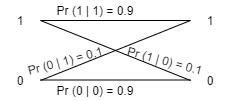
\includegraphics[width=\columnwidth]{Assignment-13/Code/Figure/Bin_Symm.png}
    \centering \caption*{Fig 1.0: Direct and Crossover Probability}
\end{figure}

Let a binomial r.v be X $\in$ $\{0, 1\}$ representing the number of bits transmitted incorrectly.
The sample space is given as $\{0, 1, 2, 3\}$.

\begin{equation}\tag{1.1}
    X \sim Bin(n=3, p=0.1)
\end{equation}
The binomial p.m.f. is given by:
\begin{equation}\tag{1.2}
    \pr{X=k} &= {n\choose k} p^{k} (1-p)^{n-k}\\
\end{equation}
Putting the values of X in (1.2) and sum up to get the probability of correct decoding,
\begin{equation}\tag{1.3}
    \begin{split}
        \pr{X=0} &= {3\choose 0} (0.1)^{0} (1-0.1)^{3-0}\\
                 &= (0.9)^{3}\\
        \pr{X=1} &= {3\choose 1} (0.1)^{1} (1-0.1)^{3-1}\\
                 &= 3\ (0.1)\ (0.9)^{2}
    \end{split}
\end{equation}
The probability of correct decoding is given by,
\begin{equation}\tag{1.4}
    \begin{split}
        P_c &= \pr{X=0} + \pr{X=1}\\
            &= (0.9)^{3} + 3\ (0.1)\ (0.9)^{2}\\
            &= 0.972\\
    \end{split}
\end{equation}
The average probability of error \\
\begin{equation}\tag{1.5}
    \begin{split}
            P_e  &= 1\ -\ P_c\\
                   &= 1\ -\ 0.972\\
                   &= 0.028
    \end{split}
\end{equation}
\end{document}
